\documentclass[11pt]{article}
\usepackage{amsmath, amsfonts, amsthm, amssymb}  % Some math symbols
\usepackage{enumerate}
\usepackage{fullpage}
\usepackage[x11names, rgb]{xcolor}
\usepackage{tikz}
\usepackage{graphicx}
\usetikzlibrary{snakes,arrows,shapes}
\usepackage{wasysym}
\usepackage{dsfont}
\usepackage{centernot}
\usepackage{float}
\usepackage[margin=0.5in]{geometry}

\setlength{\parindent}{0pt}
\setlength{\parskip}{5pt plus 1pt}
\pagestyle{empty}

\def\indented#1{\list{}{}\item[]}
\let\indented=\endlist

\newcounter{questionCounter}
\newcounter{partCounter}[questionCounter]

\newenvironment{question}[2][\arabic{questionCounter}]{%
    \addtocounter{questionCounter}{1}%
    \setcounter{partCounter}{0}%
    \vspace{.25in} \hrule \vspace{0.5em}%
        \noindent{\bf #2}%
    \vspace{0.8em} \hrule \vspace{.10in}%
}{}

\renewenvironment{part}[1][\alph{partCounter}]{%
    \addtocounter{partCounter}{1}%
    \vspace{.10in}%
    \begin{indented}%
       {\bf (#1)} %
}{\end{indented}}

%%%%%%%%%%%%%%%%% Identifying Information %%%%%%%%%%%%%%%%%
%% This is here, so that you can make your homework look %%
%% pretty when you compile it.                           %%
%%     DO NOT PUT YOUR NAME ANYWHERE ELSE!!!!            %%
%%%%%%%%%%%%%%%%%%%%%%%%%%%%%%%%%%%%%%%%%%%%%%%%%%%%%%%%%%%
\newcommand{\myname}{Michael Rosenberg}
\newcommand{\myandrew}{mmrosenb@andrew.cmu.edu}
\newcommand{\mycourse}{73-449: Social, Economic, and Information Networks}
\newcommand{\myhwname}{| Final Project Report}
\newcommand{\myrecitation}{Anderson, Section A}
\newcommand{\myteammates}{}
\newcommand{\Z}{\mathds{Z}}
\newcommand{\bigdot}{\textbf{.} }
\newcommand{\spa}{\hspace{2cm}}
\newcommand{\proposition}{\textbf{\underline{Proposition:} }}
\newcommand{\proofwrite}{\textbf{\underline{Proof.} }}
\newcommand{\claim}{\textbf{\underline{Claim.} }}
\newcommand{\AFSOC}{Assume for the sake of contradiction }
\newcommand{\theorem}{\textbf{\underline{Theorem:}} }
\newcommand{\definition}{\textbf{\underline{Definition:}} }
\newcommand{\xNot}{\mathbf{x}_0}
%%%%%%%%%%%%%%%%%%%%%%%%%%%%%%%%%%%%%%%%%%%%%%%%%%%%%%%%%%%%%%%%%%%%%%%%%%%%%%%%

\begin{document}
\begin{center}
    {\Large \mycourse} {\Large \myhwname} \\
    \myrecitation \\
    \myname \\
    \myandrew \\
    %\myteammates 
\end{center}

\subsection{Introduction}

A tax haven is a jurisdiction where individuals and companies can get a
more favorable tax rate on their assets than another
jurisdiction. Typically, a tax haven is a country with a
favorable tax regime, although it can also be a territory embeded within a
country. Individuals and companies often want to set up entities within tax
havens for two reasons. The first reason is that the tax regime within
a haven is often helpful for retaining a large amount of financial assets
for a company. The second reason is that tax havens typically have looser
laws on financial transparency when compared to other jurisdictions, and so
companies can use entities within tax havens to perform
transactions in a less regulated environment than their typical jurisdiction.

Tax havens have been a source of controversy in developed and middle-income
countries in recent years. Governments have been concerned by the many large
private institutions that choose to set up entities within tax havens such as
Switzerland, the Bahamas, and Panama. This concern comes from two issues. The
first issue is that when companies set up entities within these tax havens, a
lot of tax revenue that would come from domestic financial transactions is lost
due to the offshoring of certain business components; this is often considered
tax evasions in the eyes of governments. The other reason is that the lack of
financial transparency in these tax havens allows certain informal economies to
develop around the world, such as the financial backing of the drug trade.

Upon initial consideration of these issues, it becomes apparent that
the financial relationships formed by
domestic companies and offshore entities to be a topic for network analysis. 
My first question is, what aspects of the tax haven
network give legal and financial intermediaries social capital in the network?
If we are able to identify these aspects of the network, we would be able to
identify the responsibility that domestic intermediaries have in building
networks for tax evasion. My second question is, what are some policy
interventions we can do to reduce the strength of this network? If we begin to
build some of these policy interventions, we may be able to find mechanisms to
reduce global tax evasion and fight illicit economies.

\subsection{The Dataset}

The source of my data comes from International Consortium of Investigative
Journalists (ICIJ). ICIJ is a non-governmental organization that
connects investigative
journalists from around the world to address cross-border crime and
corruption. This organization has created the Offshore
Leaks Database, a graph database that displays the major players in the
financing and operation of tax haven entities and the relationships among these
players. This database was formed by ICIJ using three document sources. The 
first source is the Offshore (China) Leaks, a document leak in 2013
that provided information on tens of thousands of tax haven clients from 
Hong Kong and Mainland China. The second source is the Panama Papers, a leak in 
May of 2016 that featured information on individuals transacting with the
Panamanian law firm Mossack Fonseca. The last source is the Bahamas Leaks, 
a cache of
documents that was exposed in September of 2016 that contained the financial
transactions of hundreds of thousands of Bahamian entities.

The raw dataset contains $4$ different types of agents:
\begin{itemize}
    \item \textbf{Entity}: A company, trust, or fund created in a low-tax, 
        offshore jurisdiction by another agent.
    \item \textbf{Officer}: A person or company who plays a role in an offshore 
        entity.
    \item \textbf{Intermediary}: A financial or legal go-between for a given
        individual using an offshore entity.
    \item \textbf{Addresses}: An agent's postal address.
\end{itemize}
There are $281$ different relationship types represented in this database, but
this amount of relationships is mainly a result of data quality issues and are
not truly $281$ distinct relationships. For example, some of the
most common relationships in this network are disambiguation relationships, such
as ``same name as'' or ``similar address to.'' As another example, some of these
relationships need to be textually aggregated, such as when ``shareholder of''
and ``shareholder'' are represented as two different relationships when they
are in fact the same relationship.

In order to perform a meaningful analysis on this dataset, I took several steps 
to reduce this network into a more interpretable form. 
\begin{enumerate}[1.]
    \item First,
        I removed all agents who did not represent meaningful financial 
        stakeholders in the network. This meant that I had to removing all 
        addresses from the network. 
    \item I then removed all relationships that did not represent 
        business-oriented transactions. This meant deleting all edges that were
        related to disambiguation in the network.
    \item I then removed all edge types that were not in the top $20$
        edge types. Thankfully, the top $20$ edge types represented 
        $99.5\%$ of the edge type distribution after removing all 
        disambiguation edges. 
    \item I then removed all agents who were not in the largest weakly 
        connected component. This was done for the purpose of having
        interpretable metrics on distance and paths for the network.
        This largest weakly connected component
        comprised $81.53\%$ of all agents in the network after removing all
        addresses.
    \item I then collapsed all directed relationships into the undirected
        ``does business with'' relationship. This was done for the purpose of
        making our network measures as interpretable as possible. This is a
        simplification that could be altered in future research.
\end{enumerate}
This left me with an undirected network with three different agent types (
Officers, Entities, and Intermediaries) and edges representing the 
``does business with'' relationship.

\subsection{Analysis}

I was primarily interested in studying the placement of intermediaries within
the network. To answer my first question, I wanted to compare measures of
brokerage for intermediaries (i.e. betweenness centralities) with measures of
closure for intermediaries (i.e. embeddedness, clustering coefficients). Given
that intermediaries are meant to financially connect agents across many
different countries, I was expecting that intermediaries would have social 
capital from brokerage. To answer my second question, I wanted to perform 
policy interventions where I would remove certain intermediaries or 
intermediary-entity
relationships and study how the network is dismantled. I was expecting that
it would take only the removal of a few intermediaries to collapse the structure
of this network.

\subsubsection{Summary Statistics}

The network itself has around $724000$ nodes and around $910000$ edges. This
unfortunately suggested to me that some of the network measures I wanted to
calculate would be too computationally expensive for me to develop using simple
methods, and so I would need to consider certain estimation methods for those
network measures. Upon looking at the distribution of leak sources for my nodes
(see Figure 2), I see that most of my agents were found via the Panama Papers,
with still a substantial amount coming from the Bahamas Leaks and the Offshore
Leaks. We see that a really small portion of our agents are intermediaries
(see Figure 3), which is why many of the network measures we see for
intermediares are surprising given their small representation in the network.
In terms of countries and territories represented in the network (see Figure 4),
we see that some of the expected tax havens are frequent in our dataset, such
as Hong Kong (HKG), the British Virgin Islands (VGB), and Switzerland (CHE).
Interestingly, we see that about $10\%$ of our agents are from non-identifiable
countries/territories (XXX), which suggests that it may be useful to use the
structure of the network to infer the countries of these agents.

\subsubsection{Network Measures}

Interestingly, intermediaries have relatively high degree when compared to
other agents in the network (see Figure 5), which is surprising given their
small representation in the network (see Summary Statistics). This suggests that
intermediaries do direct business with many agents, which may lend some power
to intermediaries in terms of direct interaction. Due to the large nature of
the network (see Summary Statistics), I had to find a computationally reasonable
way to compute betweenness centrality for our network. I ended up using an
estimation method that sampled a couple hundred nodes in our network for
computing paths for betweenness centrality. Unfortunately, we see that
betweenness centrality is generally low across all agent types (see Figure 6).
This either suggests that our estimation was not strong, or that intermediaries
may not be essential for connecting distant communities in the network.

For studying embeddedness, I realized that calculating average link embeddedness
for a node would be computationally difficult given that some nodes have
extremely high degree (see Figure 5). Thus, I felt a simpler method for
calculating some measure of closure for a node was to study the clustering
coefficients of our agents. Interestingly, we see that all intermediaries have
a clustering coefficient of $0$ (see Figure 6). This suggests that
intermediaries are in extremely fragile parts of the network, since their
high degree can disconnect many agents if they are removed from the network. We
also see that intermediaries are only adjacent to entities in this network. I
would argue that this is partially a data quality issue, since most
intermediaries transact with entities under the request of a legal or financial
client. That being said, considering methods on how to address this data quality
issue is slightly out of the scope of this project, and may be an avenue of
future research (see Discussion).

\subsubsection{Policy Interventions}

Given the fragile nature of the current placement of intermediaries in the
network, I started to consider certain interventions in which one could
dismantle the network by taking advantage of its fragility.

At first, I considered a scenario in which the governments of the world ban
intermediaries from interacting with offshore entities. This essentially removes
all intermediaries from the network. This intervention shatters our network into
$287000$ components, with the largest connected component only contains $22\%$
of agents in the remaining network. The average degree of this network also
shifts from $2.5$ to $1.4$, which suggests that on average most agents have
fewer direct business connections than before. When we consider how extremely
disconnected our network becomes after this policy intervention, it is
apparent that if we prevent a large number of financial and legal intermediaries
from engaging with entities, we can weaken the ability of agents to interact
with many offshore tax havens. However, given the fact that it seems unrealistic
for all governments across the world to commit to a ban like this, I thought
that it would be important to consider some more realistic scenarios.

I then considered a scenario where China decides to prevent its domestic
intermediaries from interacting with offshore entities. This removes only
Chinese intermediaries from the network, which is about $5\%$ of available
intermediaries. I considered this policy because China would seem to be the
only well-represented country in this network that would have the power to
extremely regulate its financial and legal sectors.
This intervention shatters the network into $2300$ components, but $99\%$ of
the remaining agents are within the largest connected component and the average
degree in the network stays about the same. This suggests that while the
Chinese ban can dismantle the connectivity of certain parts of the network,
this ban alone does not reduce the connectivity of the network enough to reduce
the accessibility of offshore entities. This also suggests that this problem
can't be tackled by the policies of only one country.

I then considered a policy scenario where the US and the UK engage in light
regulation on the number of intermediary-entity connections per intermediary
in their country. This policy scenario caps the degree of US and UK
intermediaries at $5$, and so any intermediary in these countries that has over
$5$ adjacencies must choose which adjacencies to keep at random. This scenario
is primarily meant to see the effect of a small number of developed countries
engaging in light regulation of their financial intermediaries. This shatters
our network into $12000$ components, but $97\%$ of the remaining nodes are
within the largest connected component and the average degree only shifts
slightly from $2.45$ to $2.5$. Thus, while the multi-country effort seems to 
have damaged some parts of the Atlantic tax haven, it did not do enough
damage to the East Asian part of the network to be an extremely effective
policy.

\subsection{Discussion and Future Research}

It seems as though intermediaries have social capital in this network from
having many direct business connections with entities and being placed in very
fragile parts of the network. While these aspects of intermediaries
would suggest that their social capital cannot be characterized by closure, it
is uncertain whether intermediaries could have social capital characterized
by brokerage since our betweenness measures for intermediaries are weak (see
Analysis, Network Measures). After attempting several different types of
policy interventions, it seems as though the most effective methods for
dismantling the network was to remove a meaningful number of intermediaries
across several countries in the network. Thus, the best direction for 
policymaking on breaking up this network would be to form a strong 
multinational coalition for regulating intermediary-entity relationships.

There are several possible avenues of future research. One avenue is to study
this dataset with more computationally efficient algorithms. If we had more
resources for computing power on this large graph, many of our calculations on
embeddedness and betweenness centrality could be more accurately measured and
not simply estimated. Another avenue is to study the structure of the network
to infer what relationships exist between intermediaries and officers. Given
the peculiarity of the lack of relationships between intermediaries and officers
on this network, it may be useful to use certain statistical methods to infer
likely connections between intermediaries and their likely clients. Finally,
another avenue of research would be to build slightly more robust policy
interventions. If we were to add some level of randomness to the policy
decisions using Monte Carlo simulations, we may be able to make more meaningful
suggestions on how to dismantle the tax haven network.

\begin{figure}[H]
\centering
\begin{minipage}{.5\textwidth}
  \centering
  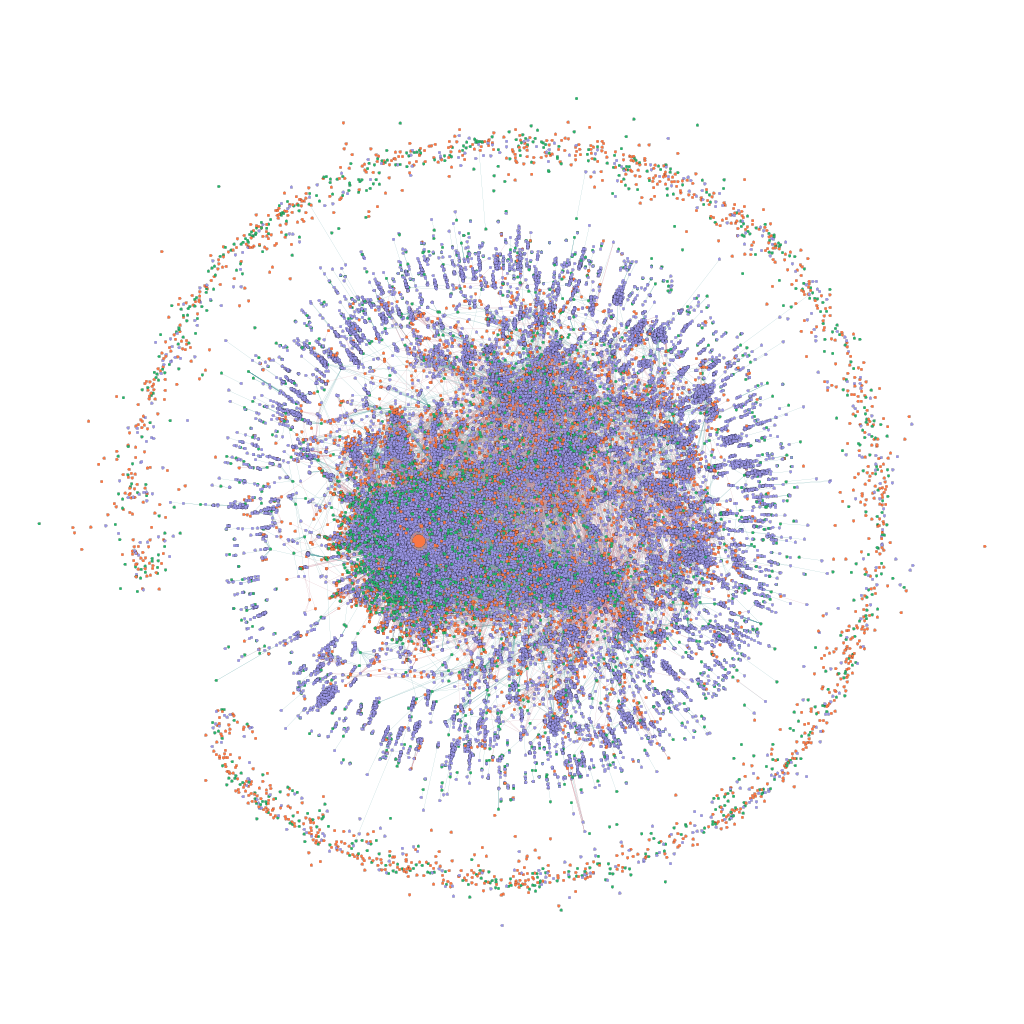
\includegraphics[width=3in]{figures/figure1.png}
  \caption{A visualization of our final dataset with the removal of
            nodes with a degree of less than $5.$ Nodes are sized by
            degree and nodes are colored by agent type, where entities are
            purple, officers are orange, and intermediaries are green.}
  \label{fig1}
\end{minipage}%
\begin{minipage}{.5\textwidth}
  \centering
  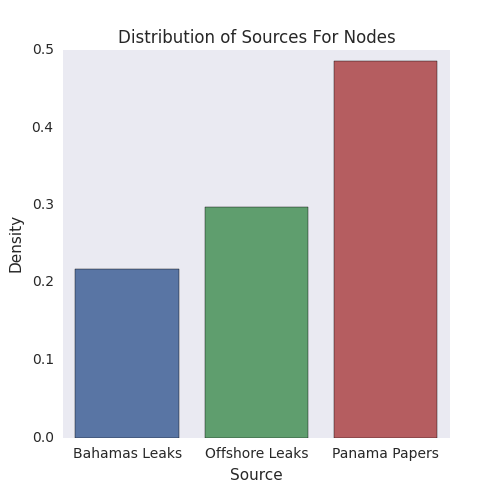
\includegraphics[width=3in]{figures/figure2.png}
  \caption{Distribution of Leak Source for nodes in the canonical
                    network.}
  \label{fig2}
\end{minipage}
\end{figure}

\begin{figure}[H]
\centering
\begin{minipage}{.5\textwidth}
  \centering
  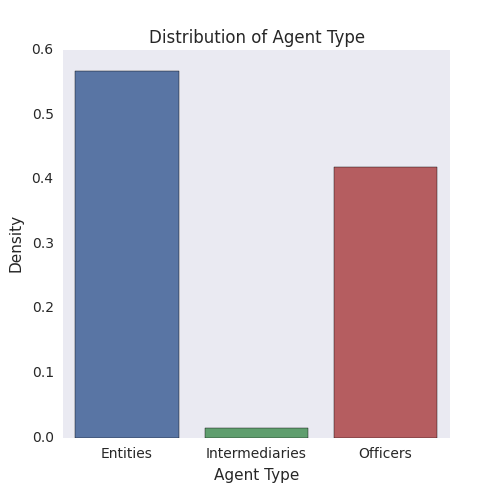
\includegraphics[width=3in]{figures/figure3.png}
  \caption{Distribution of Agent Type for nodes in the canonical network.}
  \label{fig3}
\end{minipage}%
\begin{minipage}{.5\textwidth}
  \centering
  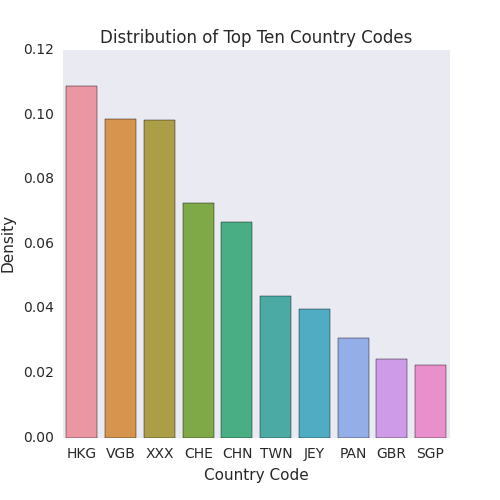
\includegraphics[width=3in]{figures/figure4.png}
  \caption{Top Ten Country Codes (For both Countries and Territories) for
                nodes in our canonical network.}
  \label{fig4}
\end{minipage}
\end{figure}

\begin{figure}[H]
\centering
\begin{minipage}{.5\textwidth}
  \centering
  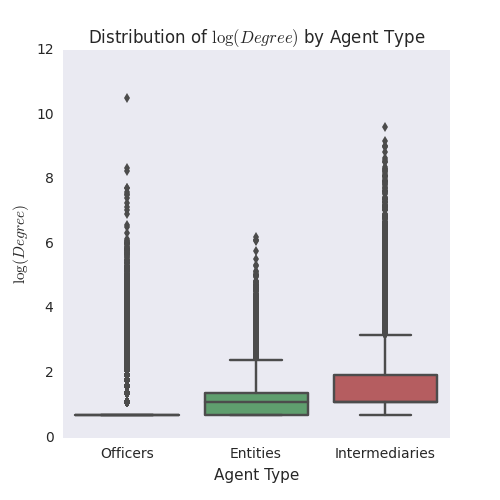
\includegraphics[width=3in]{figures/figure5.png}
  \caption{Distribution of $\log(Degree)$
        by Agent Type in the canonical network.}
  \label{fig5}
\end{minipage}%
\begin{minipage}{.5\textwidth}
  \centering
  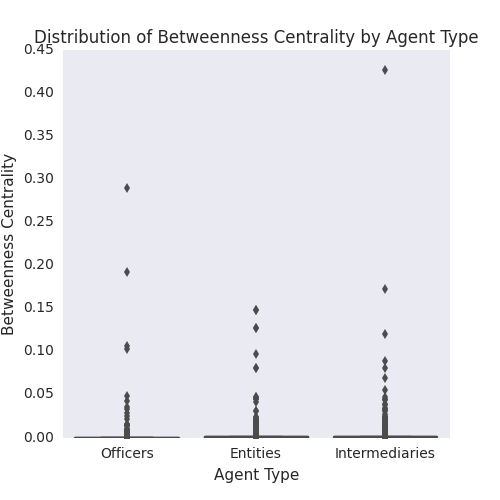
\includegraphics[width=3in]{figures/figure6.png}
  \caption{Distribution of betweenness centrality by Agent Type in the 
        canonical network.}
  \label{fig6}
\end{minipage}
\end{figure}

\begin{figure}[H]
    \centering
    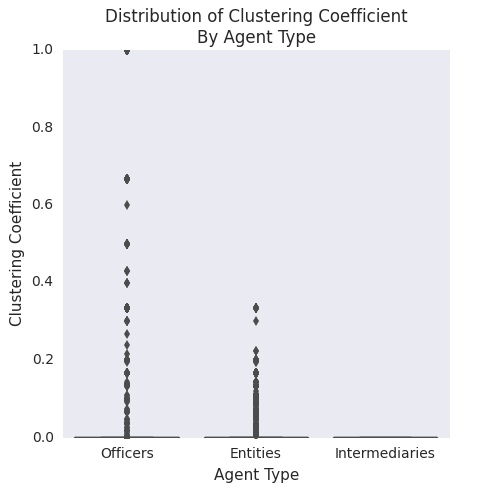
\includegraphics[width = 3in]{figures/figure7.png}
    \caption{Distribution of clustering coefficient by Agent Type in the
        canonical network.}
\end{figure}

\end{document}
